\section{Systemarkitektur}
\label{ch:Systemarkitektur}

I systemarkitekturen beskrives grænseflader for systemet og hvilke blokke det består af. Til at beskrive dette er der anvendt en række BDD'er og IBD'er. Nedenfor er de vigtigste af disse vist. For mere detaljeret beskrivelse se afsnit \ref{P-ch:SysArk} \nameref{P-ch:SysArk} på side \pageref{P-ch:SysArk} i projektdokumentationen.

\begin{figure}[h]
\centering 
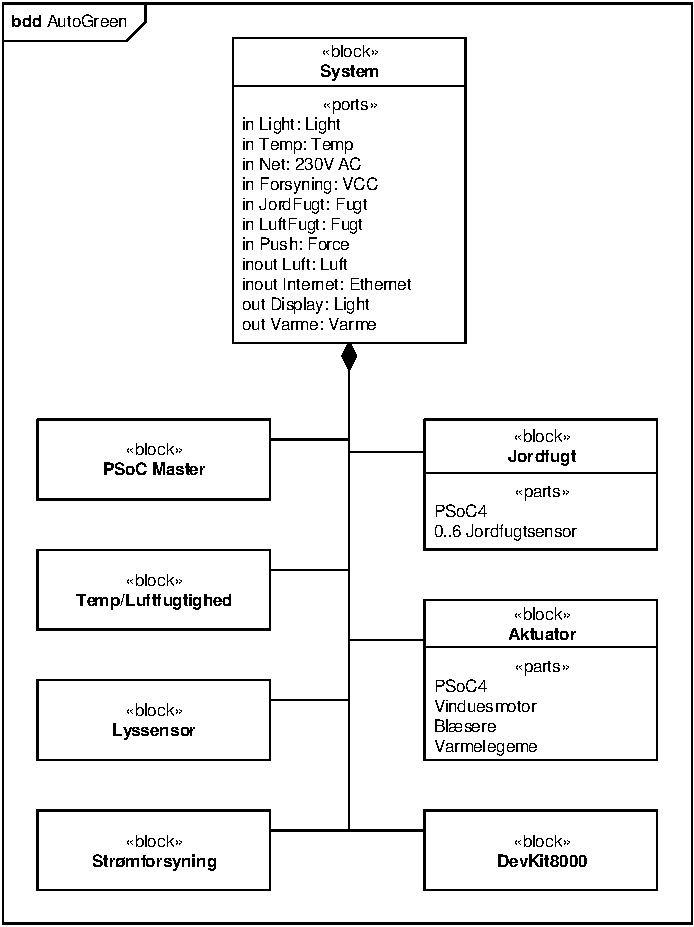
\includegraphics[scale=1.0, trim=0 0 0 0, clip=true] {../fig/bdd_system.pdf}
\caption{BDD for System.}
\label{fig:bdd_system}
\end{figure}

På Figur \ref{fig:bdd_system} kan der skabes et overblik over systemet og hvilke underblokke det består af. Det kan ses, at systemet består af syv underblokke, bl.a. PSoC Master, DevKit8000 mm. I blokken System, der består af alle de andre underblokke, vises de porte som hele systemet har, dvs. grænsefladen til omverdenen.

\clearpage

\begin{figure}[h]
\centering 
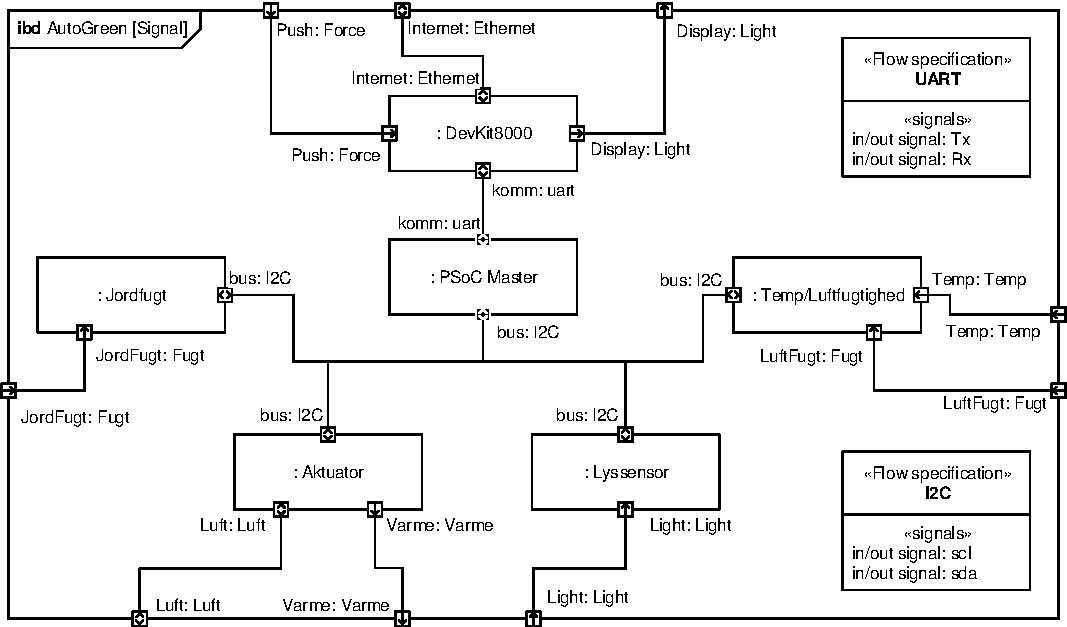
\includegraphics[scale=0.97, angle = 90] {../fig/ibd_system_signaler.pdf}
\caption{IBD for signaler i systemet.}
\label{fig:ibd_system_signal}
\end{figure}

På Figur \ref{fig:ibd_system_signal} vises alle signalerne i systemet, dvs. alle spændingsforsyninger og referencer er udeladt for overskuelighedens skyld. For at beskrive de interne signaler, tages der udgangspunkt i DevKit8000. DevKit8000 spørger løbende PSoC Master om temperatur, luftfugtighed, lysintensitet samt jordfugtighed over UART, denne er detaljeret beskrevet på side \pageref{P-sec:UART_protokol} i projektdokumentationen. Kommunikationen mellem PSoC Master, Jordfugt, Temp/Luftfugtighed, Lyssensor og Aktuator foregår over en \IIC bus. Via denne kommunikationsvej kan PSoC Master'en efterspørge alle sensorværdierne og aktivere aktuatorer, hvis DevKit8000 ønsker at regulere klimaet i drivhuset med varmelegemet, vinduet og/eller blæserne. Der kan ses en signalbeskrivelse, hvor alle signaler mellem hver blok er beskrevet i Tabel \ref{P-tbl:signalbeskriv} på side \pageref{P-tbl:signalbeskriv} i dokumentationen.

\clearpage

\begin{figure}[h]
\centering 
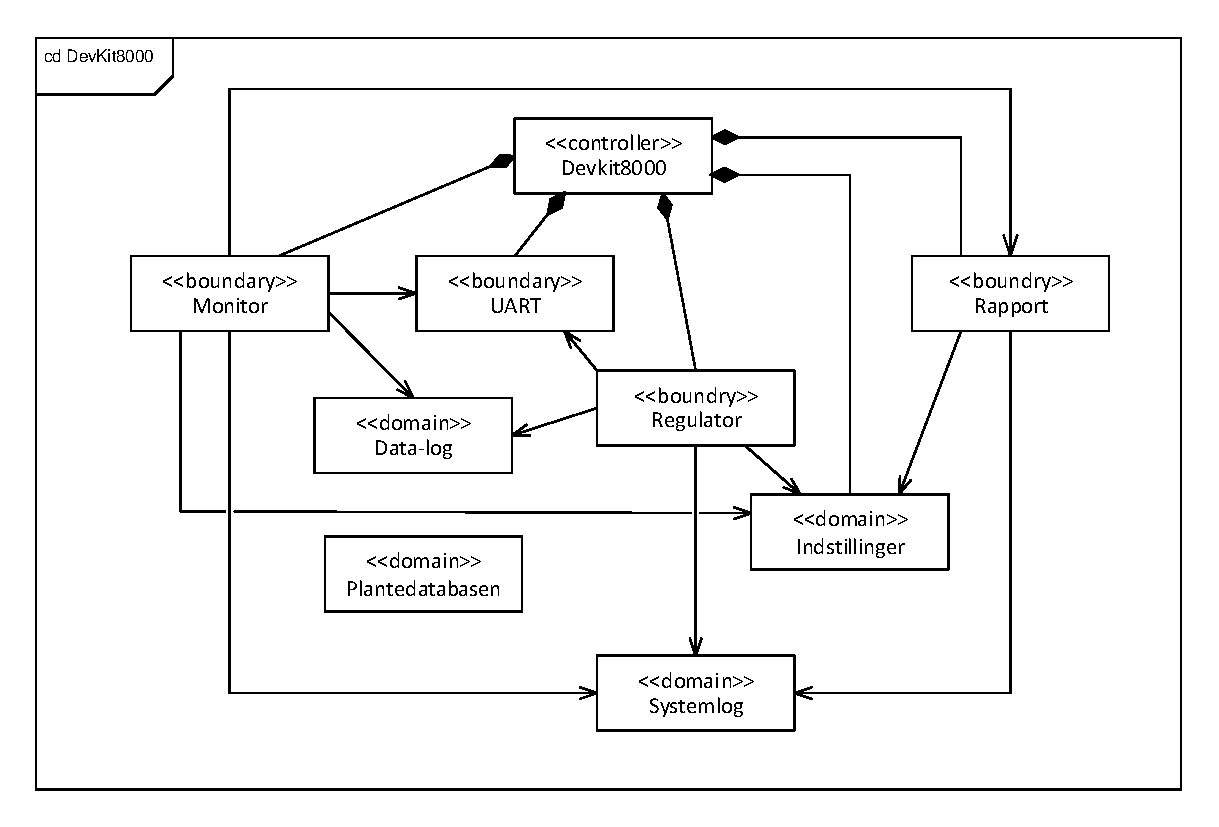
\includegraphics[scale=0.8] {../fig/UML_autogreen.pdf}
\caption{Klassediagram for DevKit8000}
\label{fig:UML}
\end{figure}

På Figur \ref{fig:UML} ses et UML klassediagram, som viser relationer mellem klasserne på DevKit8000. Der anvendes to relationstyper; komposition og association. Domain klassen datalog har til opgave at gemme de sensordata som monitor opsamler, jf. Listing \ref{P-lst:Sensordata_struct} på side \pageref{P-lst:Sensordata_struct} i dokumentationen. Regulatoren anvender denne information og bruger den til at afgøre, om forholdene i drivhuset er som ønsket. DevKit8000 er som angivet en controller klasse, og derfor binder den de øvrige klasser sammen og har den overordnede styring.

\clearpage

\begin{figure}[h]
\centering 
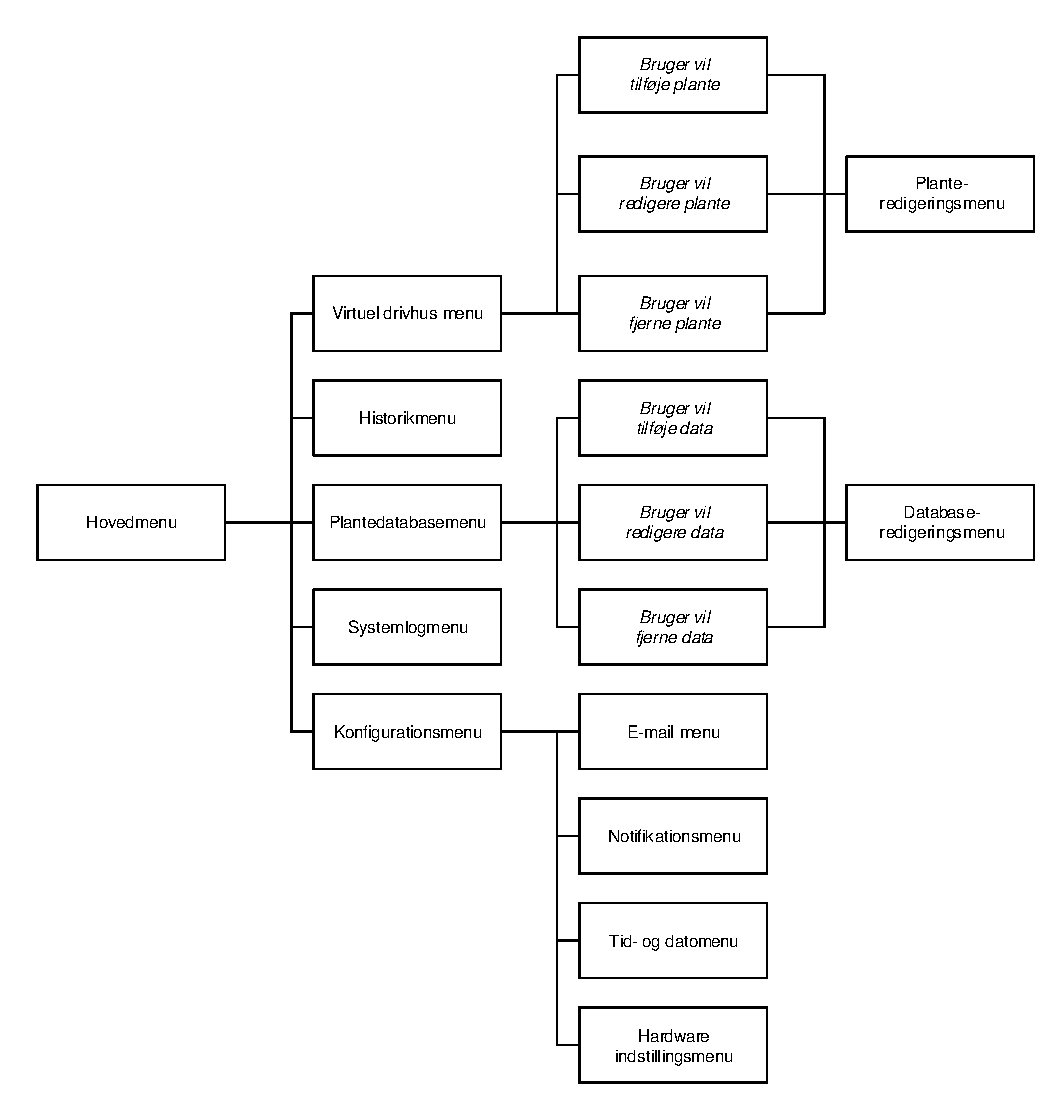
\includegraphics[width=\textwidth] {../fig/menu_oversigt.pdf}
\caption{Oversigt over AutoGreen's menuer}
\label{fig:QTMenu}
\end{figure}

Menuoversigten, der ses på Figur \ref{fig:QTMenu}, gives et samlet overblik over hvordan de forskellige menuer tilgås igennem systemet. Systemet viser altid hovedmenuen, når systemet starter op. Herfra er det muligt at få et overblik over drivhusets aktuelle klima. Hovedmenuen viser desuden fem knapper, hvor man kan få adgang til undermenuerne: virtuel drivhus-, historik-, plantedatabase-, systemlog- og konfigurationsmenu.

\clearpage